\chapter{Охрана труда и окружающей среды}
\section{Анализ условий труда}
\subsection{Обеспечение условий труда в отделе разработки программного обеспечения}
Дипломная работа посвящена разработке системы мониторинга состояния ЛА на основе алгоритмов интеллектуального анализа данных. Разработка производится на персональном компьютере и предполагает длительное пребывание за ним инженера.

Применение персонального компьютера освобождает человека от непроизводительной работы, связанной с обработкой информации, изменяет характер его труда. Однако при этом увеличивается доля умственного и нервно-напряженного труда, возрастает психоэмоциональная нагрузка. При значительной трудовой нагрузке, нерациональной организации работы и неблагоприятных факторах производственной среды быстро снижается работоспособность операторов, уменьшается производительность труда и ухудшается качество работы, может развиться перенапряжение,~а в отдельных случаях возникнуть срыв трудовой деятельности~--- дистресс.

В данном разделе проводится анализ условий труда в отделе разработки информационных систем с целью обеспечения безопасности и удобства, требуемых для работы инженера.

\subsection{Характеристика помещения}
Помещение находится в здании Московского Авиационного Института и представляет собой кафедральную лабораторию со следующими размерами:
\begin{itemize}
	\item длина~6~м;
	\item ширина~4~м;
	\item высота~3.5~м.
\end{itemize}

Площадь: $6\times4 = 24$~м\textsuperscript{2}.

Объём: $6\times4\times3,5 = 84$~м\textsuperscript{3}.

Количество рабочих мест~---~4.

Количество одновременно находящихся в помещении сотрудников не превышает~4 человек.

План помещения приведён на рисунке~\ref{fig:labourprotection:room_plan}.
\begin{figure}[h]
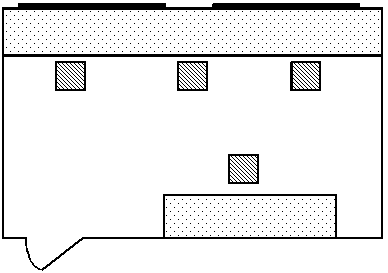
\includegraphics[width=0.6\textwidth, keepaspectratio]{plan}
\caption{План помещения}\label{fig:labourprotection:room_plan}
\end{figure}

Нормативные требования к площади и объёму рабочих мест определены в \cite{SanPin2_2_2}:
\begin{itemize}
	\item площадь на одно рабочее место с ВДТ или ПЭВМ для взрослых пользователей должна составлять не~менее~6~м\textsuperscript{2};
	\item объём~---~не~менее~20~м\textsuperscript{3}.
\end{itemize}

Фактические значения на каждого сотрудника:
\begin{itemize}
	\item площадь: $24/4 = 6$~м\textsuperscript{2};
	\item объём: $84/4 = 21$~м\textsuperscript{3}.
\end{itemize}

Данные значения показывают, что кафедральная лаборатория полностью соответствует установленным нормам.

В помещении имеются 2 оконных проёма высотой 1,6~м и шириной 2,3~м, которые выходят на юго-запад.

Искусственное освещение представляет собой 6~светильников, расположенных параллельно окнам в~2~ряда.

\subsection{Характеристика производственного процесса}
Разработка программного обеспечения производится на ПЭВМ с подключенными к ней периферийными устройствами.

\subsection{Характеристика используемого оборудования}
В процессе разработки используется следующее оборудование:
\begin{enumerate}
	\item{ПЭВМ:}
		\begin{enumerate}
			\item{процессор Intel Core i5 3,60 ГГц;}
			\item{оперативная память 8 Гб;}
			\item{жёсткий диск 1 Tб;}
			\item{напряжение питания 220 В.}
		\end{enumerate}
	\item{ЖК монитор с диагональю 23 дюйма (58,42) ASUS VX239H:}
		\begin{enumerate}
			\item{частота 75 Гц;}
			\item{яркость 250 кд/м\textsuperscript{2};}
			\item{динамическая контрастность 8 000 000 : 1;}
			\item{напряжение питания 220 В.}
		\end{enumerate}
	\item{Клавиатура Logitech K330;}
	\item{Мышь A7Tech X;}
	\item{Принтер HP LaserJet 1005M:}
		\begin{enumerate}
			\item{напряжение питания 220 В.}
		\end{enumerate}
\end{enumerate}

\subsection{Санитарно-гигиенические факторы}

\subsubsection{Микроклимат помещения}
Микроклимат в рабочем помещении должен соответствовать \cite{GOST12_1_005}.

Согласно \cite{GOST12_1_005}, работа разработчика ПО относится к категории «Легкая~–~Iа», т.к. лёгкие физические работы~--- работы с расходом энергии не более 150 ккал (174 Вт), а категория Iа подразумевает энергозатраты до 120~ккал/ч~(139 Вт).

Рабочее место разработчика ПО является постоянным, т.к. он находится на нём большую часть рабочего времени (более~50\%).

Нормативные и фактические значения для категории работ «Легкая~–~Iа», лёгкие физические работы~--–~работы с расходом энергии не более 150~ккал (174~Вт). Категория Iа подразумевает энергозатраты до 120~ккал/ч (139~Вт).

Рабочее место разработчика модели является постоянным, т.к. он находится на нём большую часть рабочего времени (более 50\%).

Нормативные и фактические значения для категории работ «Легкая – Iа» и постоянного рабочего места приведены в таблице~\ref{tab:labourprotection:microclimat}.

\begin{table}[h]
\caption{Значения характеристик микроклимата помещения}
\label{tab:labourprotection:microclimat}
\nohyphenation

\begin{tabular}{|C{92pt}|C{178.25pt}|C{101.1pt}|C{124.4pt}|}
\hline
 & Температура, \textdegree C & Относительная влажность, \% & Скорость движения, м/с \\
\hline
Допустимые значения & 22--24~–-- Холодный период \linebreak 23--25~--– Теплый период & 40--60 & 0.1 \\
\hline
Фактические значения & 22--24~–-- Холодный период \linebreak 25--30~--– Теплый период & 45--55 & <0.1 \\
\hline
\end{tabular}
\end{table}

Фактические значения параметров микроклимата данного помещения удовлетворяют допустимым значениям для холодного периода года. Во время теплого периода в помещении может преобладать повышенная температура из-за отсутствия кондиционера, который бы мог её регулировать.